% -*- coding: utf-8 -*-

\begin{chapter}{Физические параметры океана}\label{chap:3}
%\chapter{The Physical Setting}
Земля имеет форму сжатого у полюсов эллипсоида вращения с экваториальным
%% в оригинале еще "an ellipse rotated about its minor axis". Если это
%% относится к определению эллипсоида вращения, то это не принципиально, 
%% т.к. эллипс симметричен по двум осям, а если это о том, что Земля вращается
%% вокруг оси... Тоже вроде известный и без того факт.
радиусом
$$
R_e=6\,378.1349\mbox{~км (West,1982)},
$$ 
который немного больше полярного радиуса 
$$
 R_p=6\,356.7497\mbox{~км}.
$$
Эта разница образуется за
%% в оригинале This small equatorial bulge, "пучность", "горб"???
счёт вращения Земли. %% ... вокруг малой оси эллипсоида (см. выше)
%
% Earth \index{earth!radii of}is an oblate ellipsoid, an ellipse rotated about 
% its minor axis, with an equatorial radius of $R_e = 6,378.1349$ km 
% (West, 1982) slightly greater than the polar radius of $R_p = 6,356.7497$ km.
% The small equatorial bulge is due to earth's rotation.

Расстояния на земной поверхности измеряются в различных
единицах; наиболее распространёнными являются градусы широты и
долготы, метры, мили и морские мили. \emph{Широта}~--- это угол между
вертикалью на местности и экваториальной плоскостью. Меридиан~--- это
линия пересечения земной поверхности с плоскостью, перпендикулярной 
экваториальной плоскости и проходящей через ось вращения
Земли. \emph{Долгота}~--- это угол между нулевым меридианом и любым другим,
где нулевым является меридиан, проходящий через Королевскую Гринвичскую
обсерваторию в Англии. Таким образом, долгота измеряется на восток и
запад от Гринвича.
%
% Distances on earth are measured in many different units, the most common 
% are degrees of latitude or longitude, meters, miles, and nautical miles.
% \textit{Latitude}\index{latitude|textbf} is the angle between the local 
% vertical and the equatorial plane. A meridian is the intersection at earth's 
% surface of a plane  perpendicular to the equatorial plane and passing 
% through earth's axis of rotation. \textit{Longitude}\index{longitude|textbf}
% is the angle between the standard meridian and any other meridian, where 
% the standard meridian is the one that passes through a point at the
% Royal Observatory at Greenwich, England.  Thus longitude is measured 
% east or west of Greenwich.

За исключением экватора, градус широты на земной поверхности по длине
отличается от градуса долготы. Широта измеряется вдоль 
большого круга с радиусом~$R$, где $R$~--- средний радиус Земли. Долгота
измеряется на окружностях с радиусом~$R \cos(\varphi)$, где $\varphi$~--- широта. 
Таким образом, $1^\circ\mbox{~широты} = 111\mbox{~км}$, 
а~$1^\circ\mbox{~долготы} = 111\cos(\varphi)~\mbox{км}$. 
%%Когда требуется особая точность, следует учитывать и тот факт, 
%%что Земля~--- не сфера, так что широта тоже немного изменяется с удалением 
%%от экватора, но значения, приведённые здесь, вполне достаточны для наших целей.
%
% A degree of latitude is not the same length as a degree of longitude except
% at the equator. Latitude is measured along great circles with radius $R$,
% where $R$ is the mean radius of earth. Longitude is measured along circles 
% with radius $R \cos \varphi$, where $\varphi$ is latitude. Thus 
% $1^{\circ}$ latitude $ = 111$ km, and $1^{\circ}$ longitude 
% $= 111 \cos \varphi$ km.

Так как расстояние в градусах долготы не постоянно, океанографы
измеряют расстояние на картах, используя градусы широты.
%
% Because distance in degrees of longitude is not constant, oceanographers 
% measure distance on maps using degrees of latitude.

И морские мили, и метры исторически связаны с размерами Земли. В 1670~г.\
%% викарий церкви Святого Павла в Лионе 
Габриэль Мутон предложил
десятичную систему измерений, основанную на одной минуте дуги большого
круга Земли. Длина этой дуги позднее вошла в определение морской мили,
а предложение Мутона привело к созданию метрической
системы, основанной на другой единице длины~--- метре, который
первоначально предполагался равным одной десятимиллионной расстояния от
экватора до полюса вдоль Парижского меридиана. Хотя от взаимосвязи
морских миль и метров с размерами Земли вскоре отказались, ввиду её
непрактичности, погрешность приближённых значений, вычисленных таким образом,
достаточно мала. В самом деле, пусть длина меридиана%
\remark{Найденная как периметр эллипса с большой и малой полуосями, 
равными $R_e$ и~$R_p$ соответственно.} 
приближенно равна~$40\,008\mbox{~км}$. Отсюда одна десятимиллионная длины 
квадранта (дуги, составляющей четверть окружности) равна~$1.0002\mbox{~м}$.
%% на самом деле, это четверть длины периметра эллипса, НО определение квадранта
%% http://slovari.yandex.ru/dict/bse/article/00033/57200.htm
%% дается для окружности.
В случае морской мили поступаем аналогично: поделив длину меридиана 
на~$360 * 60 = 21600$~угловых минут, получаем~$1.8522\mbox{~км}$. Данное
значение очень близко к официальному определению \emph{международной морской
мили}: $1\mbox{~миля} \equiv 1.852\mbox{~км}$.
%
% Nautical miles and meters are connected historically to the size of earth. 
% Gabriel Mouton proposed in 1670 a decimal system of measurement based on 
% the length of an arc that is one minute of a great circle of earth.  
% This eventually became the nautical mile. Mouton's decimal system 
% eventually became the metric system based on a different unit of length,
% the meter, which was originally intended to be one ten-millionth 
% the distance from the Equator to the pole along the Paris meridian. 
% Although the tie between nautical miles, meters, and earth's radius was 
% soon abandoned because it was not practical, the approximations are very 
% good. For example, earth's polar circumference is approximately 40,008 km. 
% Therefore one ten-millionth of a quadrant is 1.0002 m. Similarly,
% a nautical mile should be 1.8522 km, which is very close to the official 
% definition of 
% the\index{nautical mile|textbf}\index{international nautical mile|textbf} 
% \textit{international nautical mile}: 1 nm $\equiv$ 1.8520 km.


\begin{section}{Океаны и моря}
% \section{Ocean and Seas}
Будем полагать, что существует единый мировой океан, условно поделенный
на три именованные части, также называемые <<океанами>>: Атлантический, 
Тихий и Индийский. Границы океанов задаются соглашениями, принятыми 
Международной гидрографической организацией. Моря, которые считаются 
частью океанов, определяются различными способами; мы рассмотрим два из них. 
%
% There is only one ocean. It is divided into three named parts by 
% international agreement: the Atlantic, Pacific, and Indian 
% ocean\index{ocean!defined} (International Hydrographic Bureau, 1953)%
%\index{International Hydrographic Bureau}. Seas, which are part of the ocean, 
% are defined in several ways. I consider two.


\begin{description}
\item[Атлантический Океан] (рис.~\ref{fig:atlantic}) расположен к северу от
Антарктиды и включает Арктическое море%
\remark{\label{remark:threeoceans}
Существуют различные мнения о том, следует ли считать Северный Ледовитый
океан морем в составе Атлантического океана (как это делает автор), либо 
отдельным океаном (согласно действующей в настоящий момент 3-й редакции 
стандарта Международной гидрографической организации 
\href{http://www.iho.shom.fr/publicat/free/files/S23_1953.pdf}%
{\textsl{Limits of oceans and seas}}, 
\texttt{http://www.iho.shom.fr/publicat/free/files/S23\_1953.pdf}).
}, европейское
Средиземноморье и американское Средиземноморье (Карибское
море). Границей между Атлантическим и Индийским океанами является
меридиан мыса Игольный (\latlon{20}{E}). Граница между Атлантическим и Тихим
океанами на юге~--- линия между мысом Горн и Южными Шетландскими
островами, а на севере~--- Берингов пролив, отделяющий Тихий океан от
Арктического моря, входящего в состав Атлантического океана.
%
% \textbf{The Atlantic Ocean} \index{ocean!Atlantic Ocean}extends
% northward from Antarctica and includes all of the Arctic Sea, the
% European Mediterranean, and the American Mediterranean more
% commonly known as the Caribbean sea (figure 3.1). The boundary
% between the Atlantic and Indian Ocean is the meridian of Cape
% Agulhas (20\degrees E). The boundary between the Atlantic and
% Pacific is the line forming the shortest distance from Cape
% Horn to the South Shetland Islands. In the north, the Arctic Sea
% is part of the Atlantic Ocean, and the Bering Strait is the
% boundary between the Atlantic and Pacific.

\begin{figure}[t!]
\makebox[121 mm] [c]{\includegraphics{pics/atlantic}}
\caption{Атлантический океан в равновеликой проекции Эккерта~VI. 
%% ??? гугл показывает как "равновеликая проекция", так и "равноплощадная",
%% но http://slovari.yandex.ru/dict/bse/article/00032/97700.htm
%% "В равновеликих (эквивалентных) К. п. сохраняются площади"
Глубины (в метрах) приведены согласно набору данных ETOPO~$30'$. 
Изобата~$200\m$ показывает границу континентального шельфа.}
\label{fig:atlantic}
\end{figure}
%
% \begin{figure}[t!]
% \makebox[121 mm] [c]{\includegraphics{atlantic}} \footnotesize
% \centering Figure 3.1 The Atlantic Ocean viewed with an Eckert
% VI\rule{0mm}{3ex} equal-area projection. Depths, in meters, are
% from the \textsc{etopo} 30$'$ data set. The 200 m contour outlines
% continental shelves.
%
% \label{fig:atlantic}
% \vspace{-4ex}
% \end{figure}

\item[Тихий Oкеан] (рис.~\ref{fig:pacific}) простирается к северу 
от Антарктиды до Берингова пролива. Граница между Тихим и Индийским океаном 
лежит на линии, проходящей
от Малайского полуострова через Суматру, Яву, Тимор, австралийский мыс
Лондондерри и Тасманию, а от Тасмании до Антарктиды~--- на меридиане мыса 
Северо-Восточный (\latlon{147}{E}).
%
% \textbf{The Pacific Ocean} \index{ocean!Pacific Ocean}extends
% northward from Antarctica to the Bering Strait (figure 3.2). The
% boundary between the Pacific and Indian Ocean follows the line
% from the Malay Peninsula through Sumatra, Java, Timor, Australia
% at Cape Londonderry, and Tasmania. From Tasmania to Antarctica it
% is the meridian of South East Cape on Tasmania 147\degrees E.

\begin{figure}[t!]
\makebox[121 mm] [c]{\includegraphics{pics/pacific}}
\caption{Тихий океан в равновеликой проекции Эккерта~VI. 
Глубины (в метрах) приведены согласно набору данных ETOPO~$30'$. 
Изобата~$200\m$ показывает границу континентального шельфа.}
\label{fig:pacific}
\end{figure}
%
% \begin{figure}[t!]
% \makebox[121 mm] [c]{\includegraphics{pacific}}
% \centering
% \footnotesize
% Figure 3.2 The Pacific Ocean viewed with an Eckert VI\rule{0mm}{3ex} equal-area
% projection. Depths, in meters, are from the \textsc{etopo} 30$'$ data set. The
% 200 m contour outlines continental shelves.
% 
% \label{fig:pacific}
% \vspace{-4ex}
% \end{figure}

\item[Индийский Океан] (рис.~\ref{fig:indian}) простирается от Антарктиды 
до Евразийского континента, включая в себя Красное море и Персидский залив. 
%
% \textbf{The Indian Ocean} \index{ocean!Indian Ocean}extends from
% Antarctica to the continent of Asia including the Red Sea and
% Persian Gulf (figure 3.3). Some authors use the name Southern
% Ocean to describe the ocean surrounding Antarctica.

\begin{figure}[t!]
\makebox[121 mm] [c]{\includegraphics{pics/indian}}
\caption{Индийский океан в равновеликой проекции Эккерта~VI. 
Глубины (в метрах) приведены согласно набору данных ETOPO~$30'$. 
Изобата~$200\m$ показывает границу континентального шельфа.}
\label{fig:indian}
\end{figure}
%
% \begin{figure}[t!]
% \makebox[121 mm] [c]{\includegraphics{indian}}
% \footnotesize
% \centering
% Figure 3.3 The Indian Ocean viewed with an Eckert VI\rule{0pt}{3ex}
% equal-area projection. Depths, in meters, are from the \textsc{etopo} 30$'$ 
% data set. The 200 m contour outlines continental shelves.
%
% \label{fig:indian}
% \vspace{-4ex}
% \end{figure}
\end{description}

Некоторые авторы используют название Южный океан для вод вокруг Антарктиды.%
\remark{
Южный океан включен в проект очередной, 4-й редакции стандарта 
(\href{http://www.iho-ohi.net/mtg_docs/com_wg/S-23WG/S-23WG_Misc/Draft_2002/Draft_2002.htm}%
{\texttt{http://www.iho-ohi.net/mtg\_docs/com\_wg/S-23WG/S-23WG\_Misc/Draft\_2002/Draft\_2002.htm}}).
} 

Существуют различные типы морей. Мы ограничимся двумя:
\begin{description}
\item[Средиземные моря] большей частью окружены сушей. Согласно этому
определению, Арктическое и Карибское моря~--- средиземные, Арктическое
cредиземное и Карибское cредиземное.
%
% \textbf{Mediterranean Seas} \index{seas!Mediterranean}are mostly
% surrounded by land. By this definition, the Arctic and Caribbean
% Seas are both Mediterranean Seas, the Arctic Mediterranean and the
% Caribbean Mediterranean.

\item[Окраинные моря] определяются только изрезанностью побережья.
Примерами окраинных морей являются Аравийское и Южно-Китайское моря.
%
% \textbf{Marginal Seas} \index{seas!marginal}are defined by only an
% indentation in the coast. The Arabian Sea and South China Sea are
% marginal seas.
\end{description}
\end{section}


\begin{section}{Размеры океанов}
% \section{Dimensions of the ocean}
Океаны и моря покрывают $70.8\%$~земной поверхности, что 
составляет~$361\,254\,000~\mbox{км}^2$. Площади океанов значительно 
различаются (табл.~3.1):
%
% \index{ocean!dimensions of}The ocean and seas cover 70.8\% 
% of the surface of earth, which amounts to 361,254,000 km$^2$. 
% The areas of the named parts vary considerably (table 3.1).

\begin{tabular}{lr}
%% Таблица 3.1. Площадь океанов $^{\dag }$
Тихий Океан         & $181.34 \times 10^6 \mbox{км}^2$ \\
Атлантический Океан & $106.57 \times 10^6 \mbox{км}^2$ \\
Индийский Океан     & $ 74.12 \times 10^6 \mbox{км}^2$ \\
%% $^{\dag }$ From Menard and Smith (1966)
\end{tabular}
%
% \begin{table} [b!]\centering \small
% \vspace{-3ex}
% \begin{tabular*}{65mm}{@{}l @{\extracolsep{\fill}} r@{}}
% \multicolumn{2}{@{}l@{}}{\bfseries Table 3.1 Surface Area of the ocean} $^{\dag }$ \\
% \hline
% \rule{0ex}{2.5ex}Pacific Ocean  & $181.34 \times 10^6 \hbox{ km}^2$        \\
%                  Atlantic Ocean   & $ 106.57 \times 10^6 \hbox{ km}^2$        \\
%                 Indian Ocean  & $74.12 \times 10^6 \hbox{ km}^2$        \\[0.5ex]
% \hline
% \multicolumn{2}{@{}l@{}}  {\rule{0ex}{2.5ex}$^{\dag }$ From Menard and Smith (1966)}
% \end{tabular*} \\[0.5ex]
% \vspace{-3ex}
% \end{table}


Горизонтальные размеры океанов изменяются от $1500\mbox{~км}$~--- минимальной
ширины Атлантического океана, до $13000\mbox{~км}$~--- его протяженности
с севера на юг либо ширины Тихого океана.
При этом типичные глубины составляют~$3$--$4\mbox{~км}$.
Таким образом, горизонтальные размеры океанских бассейнов в $1000\mbox{~раз}$
больше, чем вертикальные.  Масштабы Тихого океана можно представить
себе с помощью обычного листа бумаги $8.5 \times 11~\mbox{дюймов}$:
задав коэффициент масштабирования~$10\mbox{~дюймов} = 10\,000\mbox{~км}$,
получим, что ширина океана сравнима с размерами листа, а глубина 
в~$3\mbox{~км}$, которая в выбранном масштабе равна~$0.003\mbox{~дюйма}$,
соответствует типичной толщине листа.
%
% Oceanic dimensions range from around 1500 km for the minimum width of the
% Atlantic to more than 13,000 km for the north-south extent of the Atlantic 
% and the width of the Pacific. Typical depths are only 3--4 km. So horizontal
% dimensions of ocean basins are 1,000 times greater than the vertical
% dimension. A scale model of the Pacific, the size of an $8.5 \times 11$ in 
% sheet of paper, would have dimensions similar to the paper: a width 
% of 10,000 km scales to 10 in, and a depth of 3 km scales to 0.003 in, 
% the typical thickness of a piece of paper.


Таким образом, графики поперечного сечения океана для
удобства использования должны иметь сильно преувеличенный вертикальный
масштаб. Как правило, его выбирают в 200 раз большим, 
чем горизонтальный (рис.~\ref{fig:bathy}). Это преувеличение искажает наши
представления об океане. Края океанических бассейнов (континентальные
склоны), которые на рис.~\ref{fig:bathy} выглядят крутыми обрывами 
(\latlon{41}{W}, \latlon{12}{E}), на самом деле представляют собой 
пологие склоны, понижающиеся на~$1\mbox{~м}$ по вертикали 
на каждые~$20\mbox{~м}$ по горизонтали.
%
% Because the ocean is so thin, cross-sectional plots of ocean basins must 
% have a greatly exaggerated vertical scale to be useful. Typical plots have
% a vertical scale that is 200 times the horizontal scale (figure 3.4). This 
% exaggeration distorts our view of the ocean. The edges of the ocean basins, 
% the continental slopes, are not steep cliffs as shown in the figure 
% at 41\degrees W and 12\degrees E. Rather, they are gentle slopes dropping 
% down 1 meter for every 20 meters in the horizontal.

\begin{figure}[t!]
\makebox[121 mm] [c]{\includegraphics{pics/bathy}}
\caption{Профиль дна в южной Атлантике вдоль \latlon{25}{S}, демонстрирующий 
континентальный шельф Южной Америки, подводную гору (\latlon{35}{W}), 
Срединнo-Атлантический хребет (\latlon{14}{W}), 
хребет Вальвис (\latlon{6}{E}) и узкий континентальный шельф Южной Африки. 
\textbf{Вверху:} масштаб по вертикали увеличен в соотношении 180:1. 
\textbf{Внизу:} масштаб по вертикали увеличен в соотношении 30:1. 
Если нарисовать график в действительных пропорциях, то он будет тоньше, 
чем линия, обозначающая поверхность моря на нижнем графике.}
\label{fig:bathy}
\end{figure}
%
% \begin{figure}[t!]
% \makebox[121 mm] [c]{\includegraphics{bathy}}
% \footnotesize
% Figure 3.4 Cross-section of the south Atlantic\rule{0pt}{3ex} along 
% 25\degrees S showing the continental shelf offshore of South America, 
% a seamount near 35\degrees W, the mid-Atlantic Ridge near 14\degrees W, 
% the Walvis Ridge near 6\degrees E, and the narrow continental shelf off 
% South Africa. \textbf{Upper} Vertical exaggeration of 180:1. 
% \textbf{Lower} Vertical exaggeration of 30:1. If shown with true aspect 
% ratio, the plot would be the thickness of the line at the sea surface 
% in the lower plot.
% \label{fig:bathy}
% \vspace{-4ex}
% \end{figure}

Малое отношение глубин океанических бассейнов к их ширине также играет 
важную роль в теории океанских течений. Так, вертикальные скорости 
должны быть гораздо меньше, чем горизонтальные. Даже на расстояниях
порядка нескольких сотен километров вертикальные скорости должны составлять 
менее $1\%$~горизонтальных. Мы используем эту информацию позже для того, 
чтобы упростить уравнение движения.
%
% The small ratio of depth to width of the ocean basins is very important 
% for understanding ocean currents. Vertical velocities must be much smaller
% than horizontal velocities. Even over distances of a few hundred kilometers,
% the vertical velocity must be less than 1\% of the horizontal velocity.
% I will use this information later to simplify the equations of motion.

В то же время, относительно малые вертикальные скорости существенно влияют
на турбулентность. Трёхмерная турбулентность по своей природе сильно
отличается от двумерной. В двумерной турбулентности вихревые линии
всегда должны быть вертикальны, так что растяжение вихря невелико.
С другой стороны, в трёхмерном случае растяжение вихря
играет фундаментальную роль.
%
% The relatively small vertical velocities have great influence on
% turbulence\index{turbulence}. Three dimensional turbulence is fundamentally
% different than two-dimensional turbulence\index{turbulence!two dimensional}.
% In two dimensions, vortex lines must always be vertical, and there can be
% little vortex stretching. In three dimensions, vortex stretching plays
% a fundamental role in turbulence.
\end{section}

\begin{section}{Элементы рельефа}
% \section{Sea-Floor Features}
Земная кора делится на два типа: сравнительно тонкая (около~$10\mbox{~км}$), 
но более плотная океаническая и более толстая (около~$40\mbox{~км}$), но
менее плотная континентальная. Участки коры континентального типа погружаются
в более плотное вещество мантии не так глубоко, как участки океанического типа,
так что средняя высота их поверхности относительно уровня моря имеет два
различных значения: континенты в среднем возвышаются на~$1100\mbox{~м}$, 
а дно океанов погружено на~$-3400\mbox{~м}$ (рис.~\ref{fig:depth-r}).
%
% Earth's rocky surface is divided into two types: oceanic, with a thin
% dense crust about 10 km thick, and continental, with a thick light crust 
% about 40 km thick. The deep, lighter continental crust floats higher on 
% the denser mantle than does the oceanic crust, and the mean height of
% the crust relative to sea level has two distinct values: continents
% have a mean elevation of 1100 m, the ocean has a mean depth of -3400 m 
% (figure 3.5).

\begin{figure}[t!]
\makebox[121 mm][c]{\includegraphics{pics/depth-r}}
\caption{Гистограмма превышений суши и глубины дна океана в процентном 
отношении к площади Земли in 100 m intervals. Видно явное различие между
континентами и морским дном. Кривая кумулятивной плотности представляет собой
интеграл, вычисленный по гистограмме. Обе кривые построены по набору данных
ETOPO~2 George Sharman, Национальный центр геофизических данных НУОА.} 
\label{fig:depth-r}
\end{figure}
%
% \begin{figure}[t!]
% \makebox[121 mm] [c]{\includegraphics{depth-r}}
% \footnotesize
% Figure 3.5 Histogram of height\rule{0pt}{3ex} of land and depth of the sea 
% as percentage of area of earth in 100 m intervals, showing the clear 
% distinction between continents and sea floor. The cumulative frequency curve 
% is the integral of the histogram. The curves are calculated from the 
% \textsc{etopo} 2 data set by George Sharman of the \textsc{noaa} National 
% Geophysical Data Center. 
% \label{fig:depth-r}
% \vspace{-3ex}
% \end{figure}

Объём воды в океанах превышает объём океанических бассейнов, так что её часть
покрывает низменные окраины континентов. Образующиеся при этом мелководные 
моря называются континентальным шельфом. 
Ширина некоторых из них (например, Южно-Китайского моря) превосходит~$1100\km$,
а типичная глубина большинства сравнительно невелика: $50$--$100\m$.
Наиболее важными участками шельфа считаются Восточно-Китайское море, 
Берингово море, Северное море, Большая Ньюфаундлендская банка, Патагонский
шельф, Арафурское море и залив Карпентария, а также Сибирский
шельф. Мелководные моря помогают рассеиванию (диссипации) приливов,
они часто являются зонами высокой биологической продуктивности и, как правило,
входят в исключительные экономические зоны близлежащих стран.
%% ??? Grand Banks --- что имелось в виду: Большая Багамская банка 
%% (Grand Banks of Bahamas не гуглится) или
%% Grand Banks of Newfoundland 
%% http://www.britannica.com/EBchecked/topic/241118/Grand-Banks -- про нее
%% http://slovari.yandex.ru/dict/bse/article/00009/46500.htm -- она же
%
% The volume of the water in the ocean exceeds the volume of the ocean basins, 
% and some water spills over on to the low lying areas of the continents. These
% shallow seas are the continental shelves. Some, such as the South China Sea,
% are more than 1100 km wide. Most are relatively shallow, with typical depths 
% of 50--100 m. A few of the more important shelves are: the East China Sea,
% the Bering Sea, the North Sea, the Grand Banks, the Patagonian Shelf,
% the Arafura Sea and Gulf of Carpentaria, and the Siberian Shelf. The shallow
% seas help dissipate tides, they are often areas of high biological
% productivity, and they are usually included in the exclusive economic zone
% of adjacent countries.

Земная кора разделена на большие плиты, которые движутся относительно
друг друга. Новая кора создаётся в срединно-океанических хребтах, а
старая исчезает в глубоководных желобах. Относительное движение
литосферных плит порождает большое количество элементов морского
%% ??? due to plate tectonics "тектоника плит" --- это название геол. теории?
%% или еще и "процесса движения и деформации"?
дна. Эти элементы, изображённые на рис.~\ref{fig:bathysketch}, включают в себя
срединно-океанические хребты, глубоководные желоба, котловины и островные дуги.
Названия элементов рельефа морского дна утверждены Международной
гидрографической организацией, а определения, приведенные ниже, даются 
согласно работам Sverdrup, Johnson, and Fleming (1942), Shepard (1963)
и~Dietrich et al. (1980).
%
% The crust is broken into large plates that move relative to each other. New
% crust is created at the mid-ocean ridges, and old crust is lost at trenches.
% The relative motion of crust, due to plate tectonics, produces the
% distinctive features of the sea floor sketched in figure 3.6, including
% mid-ocean ridges, trenches, island arcs, and basins. 
% \index{ocean!features of|(}The names of the sub-sea features have been
% defined by the International Hydrographic
% Organization\index{International Hydrographic Bureau} (1953), and
% the following definitions are taken from Sverdrup, Johnson, 
% and Fleming (1942), Shepard (1963), and Dietrich et al. (1980).

\begin{figure}[b!]
\makebox[121 mm][c]{\includegraphics{pics/bathysketch}}
\caption{Схематический разрез океана, демонстрирующий основные элементы рельефа
океанского дна. Отметим, что уклоны изображены в утрированном масштабе.}
\label{fig:bathysketch}
\end{figure}
%
% \begin{figure}[b!]
% \centering
% \vspace{-2ex}
% \makebox[121 mm] [c]{\includegraphics{bathysketch}}
% \footnotesize
% Figure 3.6 Schematic section through the ocean showing\rule{0pt}{4ex} 
% principal features of the sea floor. Note that the slope of the sea floor 
% is greatly exaggerated in the figure.
% \label{fig:bathysketch}
% %\vspace{-4ex}
% \end{figure}

\begin{description}
\item[Котловина] 
Понижение морского дна, напоминающее по своей форме круг или овал.
%
% \textit{Basins} \index{basins|textbf}are deep depressions of the sea floor
% of more or less circular or oval form.

\item[Каньон]
Относительно узкая глубокая долина с крутыми склонами, проходящая по
континентальному шельфу и континентальному склону, глубина
которой постоянно увеличивается.
%% "долина" отсюда: http://slovari.yandex.ru/dict/gl_natural/article/3004/300_4104.HTM
%% из формулировки неясно, вдоль или поперек шельфа идет
%% еще определение: http://slovari.yandex.ru/dict/bse/article/00032/20400.htm
%
% \textit{Canyons} \index{canyon|textbf}are relatively narrow, deep furrows 
% with steep slopes, cutting across the continental shelf and slope, with
% bottoms sloping continuously downward.

\item[Континентальный шельф]
Зона, смежная с континентом (или окружающая остров), простирающаяся от
линии малой воды до глубины (как правило, порядка~$120\m$), на которой
%% ??? линии наибольшего отлива, уреза малой воды, и т.п.
%% http://www.multitran.ru/c/m.exe?l1=1&l2=2&s=low-water+line
%% первоначальный вариант перевода содержал термин "горизонт меженных вод"
%% но это вроде (http://slovari.yandex.ru/dict/bse/article/00046/79300.htm)
%% относится к рекам и сезонным изменениям, а не к приливам/отливам
обнаруживается резкое или хотя бы достаточно ярко выраженное увеличение 
крутизны склона в направлении больших глубин (рис.~\ref{fig:canyon}).
%
% \textit{Continental shelves} \index{continental shelves|textbf}are zones 
% adjacent to a continent (or around an island) and extending from
% the low-water line to the depth, usually about 120 m, where there is a marked
% or rather steep descent toward great depths. (figure 3.7)

\begin{figure}[b!]
\makebox[121 mm][c]{\includegraphics{pics/canyon}}
\caption{Пример континентального шельфа~--- шельф у побережья Монтерея
в Калифорнии; здесь можно видеть каньон Монтерей и другие. Каньоны
часто встречаются на шельфе и обычно простираются через весь шельф и
континентальный склон. Права на рисунок принадлежат Monterey Bay
Aquarium Research Institute (MBARI).}
\label{fig:canyon}
\end{figure}
%
% \begin{figure}[b!]
% \vspace{-2ex}
% \makebox[121 mm] [c]{\includegraphics{canyon}}
% \footnotesize
% Figure 3.7 An example of a continental shelf,\rule{0pt}{3ex} the
% shelf offshore of Monterey California showing the Monterey and other
% canyons.  Canyons are common on shelves, often extending across the shelf 
% and down the continental slope to deep water. Figure copyright Monterey
% Bay Aquarium Research Institute (\textsc{mbari}).
% \label{fig:canyon}
% %\vspace{-3ex}
% \end{figure}
 
\item[Континентальный склон]
Уклон в сторону моря от границы шельфа к большим глубинам.
%
% \textit{Continental slopes} \index{continental slopes|textbf}are
% the declivities seaward from the shelf edge into greater depth.

\item[Равнина]
Плоская поверхность океанского дна, обнаруженная во многих глубоких бассейнах.
%
% \textit{Plains} \index{plains|textbf}are very flat surfaces found in many
% deep ocean basins.

\item[Хребет]
Вытянутое узкое поднятие морского дна с крутыми склонами и
неравномерной (нерегулярной) топографией.
%
% \textit{Ridges} \index{ridges|textbf}are long, narrow elevations of the sea
% floor with steep sides and rough topography.

\item[Подводная гора]
Изолированное или относительно изолированное поднятие, возвышающееся
на~$1000\m$ и более над дном океана, со сравнительно небольшой площадью 
вершины (рис.~\ref{fig:wildeguyot}).
%
% \textit{Seamounts} \index{seamounts|textbf}are isolated or comparatively
% isolated elevations rising 1000 m or more from the sea floor and with small
% summit area (figure 3.8).

\begin{figure}[t!]
\makebox[121 mm] [c]{\includegraphics{pics/wildeguyot}}
\caption{Пример подводной горы~--- гайот Вилд. Гайот~--- это морская гора 
с плоской вершиной. Такая форма объясняется волновым воздействием в то время, 
когда вершина горы еще находилась над уровнем моря. Поскольку подводная гора
перемещается вместе с литосферными плитами, она постепенно движется в сторону
увеличивающихся глубин. Для построения изобат использованы данные 
эхолотирования, полученные по курсу движения судна (тонкие прямые линии),
дополненные показаниями гидролокатора бокового обзора. Глубины приведены в
сотнях метров. (По данным William Sager, Texas A\&M University.)}
\label{fig:wildeguyot}
\vspace{-3ex}
\end{figure}
%
% \begin{figure}[t!]
% \makebox[121 mm] [c]{\includegraphics{wildeguyot}}
% \footnotesize
% Figure 3.8 An example of a seamount, the Wilde Guyot.\rule{0pt}{4ex} 
% A guyot is a seamount with a flat top created by wave action when the
% seamount extended above sea level. As the seamount is carried by plate
% motion, it gradually sinks deeper below sea level. The depth was contoured
% from echo sounder data collected along the ship track (thin straight lines)
% supplemented with side-scan sonar data. Depths are in units of 100 m.
% From William Sager, Texas A\&M University.
% \label{fig:wildeguyot}
% \vspace{-3ex}
% \end{figure}

\item[Разлом]
Наиболее глубокий участок хребта, отделяющего океанические котловины друг от 
друга или от близлежащего морского дна.
%
% \textit{Sills} \index{sills|textbf}are the low parts of the ridges separating
% ocean basins from one another or from the adjacent sea floor.

\item[Глубоководный желоб (впадина)]
Протяжённое, узкое и глубокое понижение морского дна с относительно
крутыми склонами (рис.~\ref{fig:aleutiantrench}).
%
% \textit{Trenches} \index{trenches|textbf}are long, narrow, and deep
% depressions of the sea floor, with relatively
% steep sides (figure 3.9).\index{ocean!features of|)}

\begin{figure}[t!]
\makebox[121 mm] [c]{\includegraphics{pics/aleutiantrench}}
\caption{Пример глубоководного жёлоба~--- Алеутский желоб;
островная дуга, п-ов Аляска и континентальный шельф, Берингово море.
Островная дуга состоит из вулканов, образовавшихся тогда, когда
океаническая кора, погружаясь в желоб, плавилась и поднималась к
поверхности.
\textbf{Вверху:} карта региона Алеутских островов в северной части Тихого 
океана.
\textbf{Внизу:} профиль через регион.}
\label{fig:aleutiantrench}
\end{figure}
%
% \begin{figure}[t!]
% \makebox[121 mm] [c]{\includegraphics{aleutiantrench}}
% \footnotesize
% Figure 3.9 An example of a trench, \rule{0pt}{3ex}the Aleutian Trench; 
% an island arc, the Alaskan Peninsula; and a continental shelf, the Bering
% Sea. The island arc is composed of volcanos produced when oceanic crust
% carried deep into a trench melts and rises to the surface.
% \textbf{Top:} Map of the Aleutian region of the North Pacific.
% \textbf{Bottom:} Cross-section through the region.
% \label{fig:aleutiantrench}
% \vspace{-4ex}
% \end{figure}
\end{description}

Элементы подводного рельефа оказывают важное влияние на циркуляцию
океанов. Хребты разделяют глубинные воды океанов на отдельные котловины. 
Вода, находящаяся глубже разлома, не
может перемещаться из одной котловины в другую. Десятки тысяч
изолированных пиков, подводных гор, разбросаны по дну океана. Они
преграждают путь течениям и вызывают турбулентность, которая приводит
к вертикальному перемешиванию вод.
%
% Sub-sea features strongly influences the ocean circulation.
% Ridges separate deep waters of the ocean into distinct basins.
% Water deeper than the sill\index{sills} between two basins cannot move
% from one to the other. Tens of thousands of seamounts are scattered
% throughout the ocean basins. They interrupt ocean currents, and produce
% turbulence\index{turbulence!in deep ocean} leading to vertical
% mixing\index{mixing!vertical} in the ocean.
\end{section}

\begin{section}{Измерение глубины океана}
% \section{Measuring the Depth of the Ocean}
Глубина океана может быть измерена двумя способами: 1) эхолотом,
установленным на судне, или 2) спутниковым альтиметром.
% The depth of the ocean is usually measured two ways: 1) using acoustic
% echo-sounders on ships, or 2) using data from satellite altimeters.

\begin{paragraph}{Эхолоты.}
Большинство карт океана созданы на основе измерений, сделанных при помощи
эхолотов. Этот прибор посылает звуковой импульс частотой
$10$--$30\kHz$ и принимает сигнал, отражённый от морского дна. Временной
интервал между посылкой импульса и приходом эха, умноженный на скорость
звука, даёт удвоенную глубину океана (рис.~\ref{fig:Sonar}).
%
% \paragraph{Echo Sounders} \index{echo sounders|(}Most maps of the ocean
% are based on measurements made by echo sounders. The instrument transmits
% a burst of 10--30 kHz sound\index{sound!used to measure depth} and listens
% for the echo from the sea floor. The time interval between transmission
% of the pulse and reception of the echo, when multiplied by the velocity
% of sound, gives twice the depth of the ocean (figure 3.10).

\begin{figure}[t!]
\makebox[121 mm] [c] {\includegraphics{pics/Sonar}}
\caption{\textbf{Слева:} Эхолокаторы измеряют глубину океана, посылая звуковой 
импульс и измеряя время, которое требуется для получения ответного сигнала, 
отраженного от дна.
\textbf{Справа:} время регистрируется при помощи искры, прожигающей отметку на
медленно движущейся бумажной ленте Dietrich et al. (1980: 124).}
\label{fig:Sonar}
\end{figure}
%
% \begin{figure}[t!]
% \makebox[121 mm] [c] {\includegraphics{Sonar}}
% %\centering
% \footnotesize
% Figure 3.10 \textbf{Left:} Echo \rule{0ex}{5ex}sounders measure depth of 
% the ocean by transmitting pulses of sound\index{sound!used to measure depth} 
% and observing the time required to receive the echo from the bottom.
% \textbf{Right:} The time is recorded by a spark burning a mark on a slowly
% moving roll of paper. After Dietrich et al. (1980: 124).
% \label{fig:Sonar}
% \vspace{-3ex}

Впервые трансатлантическое эхолотирование было выполнено в 1922~г.\ %
американским эсминцем <<Стюарт>>, 
а первые систематические промеры производились немецким
исследовательским судном <<Метеор>> в ходе экспедиции в южную
Атлантику в~1925--1927~гг. В настоящее время океанографические и военные суда
во время плавания ведут эхолотирование практически непрерывно.
Миллионы миль профилей глубины, записанных на бумагу,
%% ship-track = "морской профиль"
%% (http://www.multitran.ru/c/m.exe?CL=1&l1=1&s=ship-track),
%% но "профиль глубины" точнее в данном контексте?
были оцифрованы и занесены в базы данных, на основе которых и
составляются батиметрические карты. Распределение судовых маршрутов по
поверхности океана неравномерно. В южном полушарии они пролегают
довольно далеко друг от друга даже возле Австралии 
(рис.~\ref{fig:shiptracks10}), а в уже хорошо картированных районах, 
таких как Северная Атлантика, достаточно близко.
%
% The first transatlantic echo soundings were made by the U.S. Navy
% Destroyer \textit{Stewart} in 1922. This was quickly followed by
% the first systematic survey of an ocean basin, made by the German
% research and survey ship \textit{Meteor} during its expedition to
% the south Atlantic from 1925 to 1927. Since then, oceanographic
% and naval ships have operated echo sounders almost continuously
% while at sea. Millions of miles of ship-track data recorded on
% paper have been digitized to produce data bases used to make maps.
% The tracks are not well distributed. Tracks tend to be far apart
% in the southern hemisphere, even near Australia (figure 3.11) and
% closer together in well mapped areas such as the North
% Atlantic.\index{echo sounders|)}

\begin{figure}[t!]
\makebox[121 mm][c]{\includegraphics{pics/shiptracks10}}
\caption{Расположение данных эхолотирования, использованных для картирования 
океана около Австралии. Отметим наличие обширных пространств, в которых 
не проводились измерения с судов. 
(David Sandwell, Scripps Institution of Oceanography.)}
\label{fig:shiptracks10}
\end{figure}
%
% \begin{figure}[t!]
% %\vspace{-3ex}
% \makebox[121 mm] [c]{\includegraphics{shiptracks10}}
% \footnotesize
% %\centering
% Figure 3.11  Locations of \rule{0pt}{5ex}echo-sounder data
% used for mapping the ocean floor near Australia. Note the large areas
% where depths have not been measured from ships. From David Sandwell, 
% Scripps Institution of Oceanography.
% 
% \label{fig:shiptracks10}
% \vspace{-3ex}
% \end{figure}


%% Этот фрагмент отсутствует в оригинале, но содержит весьма полезную
%% информацию. Даже жаль выкидывать.
%%Измерения глубин эхолотированием широко используются, но у этого
%%метода есть свои ошибки.
%%\begin{enumerate}
%%\item
%%Скорость звука изменяется на $\pm 4\mbox{\%}$ в разных районах
%%океана. Используя таблицы средних скоростей звука можно уменьшить
%%ошибку измерений до $\pm 1\mbox{\%}$. Смотри параграф 3,6 для большей
%%информации о звуке в океане.
%%
%%\item
%%От малых глубин эхо может прийти не точно под корабль, а на его
%%борт. Это может вызвать небольшие ошибки в холмистых районах.
%%
%%\item
%%Местоположение корабля плохо определялось до появления в шестидесятых
%%спутниковой навигации. Ошибки могли составлять десятки километров
%%особенно в облачных регионах где невозможны астрономические
%%наблюдения.
%% 
%%\item
%%Иногда скопления зоопланктона и косяки рыбы в неглубоких райнонах
%%вызывали ошибки, приводившие к появлению на некоторых батиметрических
%%картах ложных подводных гор. Эта ошибка устраняется путём повторного
%%исследования спорных мест.
%%
%%\item
%%Некоторые районы океана (размером до 500 километров) ни разу не были
%%исследованы эхолокаторами. Это создаёт значительные пробелы в наших
%%знаниях об океанских глубинах
%%\end{enumerate}

Использование эхолотов дает наиболее точные данные о глубине океана:
их погрешность составляет~$\pm1$\%.
% Echo sounders \index{echo sounders!errors in measurement}make the most 
% accurate measurements of ocean depth.
% Their accuracy\index{accuracy!echo sounders} is $\pm$1\%.
\end{paragraph}

\begin{paragraph}{Спутниковая альтиметрия.}
Пробелы в наших знаниях о глубинах океана между маршрутами судов
теперь заполнены данными спутниковой альтиметрии. Альтиметры измеряют
(профилируют) форму морской поверхности, которая некоторым образом 
связана с рельефом дна. Чтобы понять, почему это
происходит, мы вначале должны обсудить то, как гравитация влияет на
уровень моря.
%
% \paragraph{Satellite Altimetry}
% \index{satellite altimetry!use in measuring depth} Gaps in our knowledge
% of ocean depths between ship tracks have now been filled
% by satellite-altimeter data. Altimeters profile the shape of the sea surface,
% and its shape is very similar to the shape of the sea floor
% (Tapley and Kim, 2001; Cazenave and Royer, 2001; Sandwell and Smith, 2001).
% To see this, we must first consider how gravity influences sea level.

\begin{subparagraph}{Взаимосвязь уровня моря и рельефа дна.}
% \textit{The Relationship Between Sea Level and the Ocean's Depth}
Избыток массы на дне океана, например подводная гора, увеличивает местную
гравитацию. Плотность скальных пород, образующих гору, в три раза превышает
плотность воды, поэтому масса горы соответственно больше массы воды, 
которую она замещает. В свою очередь, увеличение силы тяжести притягивает 
к горе воду, изменяя форму морской поверхности (рис.~\ref{fig:geoidsketch}).
%
% Excess mass at the sea floor, for example the mass of a seamount, increases
% local gravity because the mass of the seamount is larger than the mass
% of water it displaces. Rocks are more than three times denser than water.
% The excess mass increases local gravity, which attracts water toward
% the seamount. This changes the shape of the sea surface (figure 3.12).

\begin{figure}[t!]
\makebox[118mm][c]{\includegraphics{pics/geoidsketch}}
\caption{Плотность пород, из которых состоят подводные горы, гораздо выше,
чем плотность морской воды, поэтому их присутствие увеличивает локальную силу 
тяжести, так что локальные вертикали, определенные с помощью отвеса и 
показанные на рисунке стрелками, будут отклоняться в сторону горы. 
Поскольку поверхность океана в спокойном состоянии должна быть перпендикулярна 
силе тяжести, то поверхность моря и геоид в этом месте должны иметь 
небольшую выпуклость, как показано на рисунке. Такие выпуклости 
легко измеряются спутниковыми альтиметрами. Следовательно, данные альтиметров 
могут использоваться для картирования морского дна. Отметим, что
выпуклость поверхности моря на рисунке сильно преувеличена: подводная
гора высотой~$2\km$ порождает выпуклость высотой приблизительно~$10\m$.}
\label{fig:geoidsketch}
\end{figure}
%
% \begin{figure} [t!]
% \fbox{\parbox{12cm}{
% \centering
% \vspace{-0.5 em}
% \section*{The Geoid}
% \begin{minipage}{11.5cm}
%% ... Contents of "The Geoid" box are skipped
% \makebox[118mm][c]{\includegraphics{geoidsketch}}
% \footnotesize
% Figure 3.12 Seamounts \rule{0mm}{6ex}are more dense than sea water. They
% increase local gravity, causing a plumb line at the sea surface (arrows)
% to be deflected toward the seamount. Because the surface of an ocean at 
% rest must be perpendicular to gravity, the sea surface and the local
% geoid\index{geoid} must have a slight bulge as shown. Such bulges are 
% easily measured by satellite altimeters. As a result, satellite altimeter
% data can be used to map the sea floor. Note, the bulge at the sea surface
% is greatly exaggerated, a two-kilometer high seamount would produce a bulge
% of approximately 10 m.
% \label{fig:geoidsketch}
% \vspace{0.7ex}
% \end{minipage}
% }}
% \vspace{-4ex}
% \end{figure}

Рассмотрим это явление более подробно. С достаточной точностью можно считать, 
что поверхность моря~--- частный случай уровенной поверхности, называемой
%% ??? "поверхность уровня" или "эквипотенциальная поверхность"
%% (http://www.multitran.ru/c/m.exe?CL=1&l1=1&s=level+surface)
%% звучит лучше, но похоже, что "Уровенная поверхность"
%% как раз и есть геодезический термин: 
%% http://slovari.yandex.ru/dict/bse/article/00082/56900.htm
%% но звучит некрасиво :-(
\emph{геоидом} (см. врезку). По определению, уровенная поверхность 
представляет собой множество точек с одинаковым гравитационным потенциалом
и в каждой своей точке перпендикулярна силе тяжести. 
В частности, она должна быть перепендикулярна локальной вертикали, определяемой
при помощи \emph{отвеса}, то есть <<небольшого груза, свободно подвешенного 
на нити, по которой определяют вертикальное направление>> (Толковый словарь 
русского языка Ушакова%
\remark{
\href{http://slovari.yandex.ru/dict/ushakov/article/ushakov/15-2/us290207.htm}%
{\texttt{http://slovari.yandex.ru/dict/ushakov/article/ushakov/15-2/us290207.htm}}%
}).
%
% Let's make the concept more exact. To a very good approximation, 
% the sea surface is a particular \textit{level surface}
% \index{level surface|textbf}called the \textit{geoid} (see box).
% By definition a level surface is a surface of constant gravitational
% potential, and it is everywhere perpendicular to gravity. In particular,
% it must be perpendicular to the local vertical determined by a plumb line,
% which is ``a line or cord having at one end a metal weight for determining
% vertical direction'' (Oxford English Dictionary).

Избыток массы подводной горы притягивает грузик отвеса, тем самым немного 
отклоняя его нить от направления к центру масс Земли в сторону
горы. Так как поверхность моря должна быть перепендикулярна вектору силы
тяжести, над подводной горой образуется небольшая вспученность,
как показано на рис.~\ref{fig:geoidsketch}. Обычные подводные горы вызывают
%% Предложение "If there were no bulge, the sea surface would not be
%% perpendicular to gravity." выкинуто, поскольку фактически повторяет 
%% предыдущее.
вспученности высотой~$1$--$20\m$ на расстоянии~$100$--$200\km$. Конечно, такое
изменение высоты слишком мало, чтобы быть обнаруженным с корабля, однако
спутниковым альтиметром это сделать довольно просто. Глубоководные желоба 
вызывают дефицит масс и создают понижения морской поверхности.
%
% The excess mass of the seamount attracts the plumb line's weight, causing
% the plumb line to point a little toward the seamount instead of toward
% earth's center of mass. Because the sea surface must be perpendicular
% to gravity, it must have a slight bulge above a seamount as shown
% in figure 3.12. If there were no bulge, the sea surface would not be
% perpendicular to gravity. Typical seamounts produce a bulge that is 1--20 m
% high over distances of 100--200 kilometers. This bulge is far too small
% to be seen from a ship, but it is easily measured by satellite altimeters.
% Oceanic trenches have a deficit of mass, and they produce a depression
% of the sea surface.

Взаимосвязь между формой морской поверхности и глубиной не очень
строга. Она зависит от плотности подстилающей коры, возраста элементов рельефа, 
толщины слоя осадочных пород. 
Если подводная гора <<плавает>> на поверхности дна,
словно лёд на воде, то гравитационный сигнал будет слабее, чем если бы
она покоилась на дне, как лёд, лежащий на столе. В результате
взаимосвязь силы тяжести и рельефа дна изменяется от места к месту.
%
% The correspondence between the shape of the sea surface and the depth
% of the water is not exact. It depends on the strength of the sea floor,
% the age of the sea-floor feature, and the thickness of sediments.
% If a seamount floats on the sea floor like ice on water, the gravitational
% signal is much weaker than it would be if the seamount rested on the sea
% floor like ice resting on a table top. As a result, the relationship
% between gravity and sea-floor topography varies from region to region.

Глубина, измеряемая эхолотами, используется для того, чтобы определить
эту взаимосвязь. Затем с помощью альтиметрии проводится интерполяция
между измерениями эхолотов (Smith and Sandwell, 1994). 
%% Используя этот способ, можно расчитать
%% глубины океана с точностью до $\pm 100$~метров.
%
% Depths measured by acoustic echo sounders are used to determine the regional
% relationships. Hence, altimetry is used to interpolate between acoustic echo
% sounder measurements (Smith and Sandwell, 1994).
\end{subparagraph}

\begin{subparagraph}{Системы спутниковой альтиметрии.}
Рассмотрим, каким образом альтиметры измеряют форму земной
поверхности. Системы спутниковой альтиметрии включают в себя радар для
измерения высоты спутника над земной поверхностью и систему слежения
для определения высоты спутника в геоцентрической системе
координат. Система измеряет превышение уровня моря относительно центра
масс Земли (рис.~\ref{fig:altimetersketch}) и, тем самым, определяет 
форму морской поверхности.
%
% \textit{Satellite-altimeter systems}
% \index{satellite altimetry!systems|textbf}Now let's see how altimeters
% measure the shape of the sea surface. Satellite altimeter systems include
% a radar to measure the height of the satellite above the sea surface and
% a tracking system to determine the height of the satellite in geocentric
% coordinates. The system measures the height of the sea surface relative
% to the center of mass of earth (figure 3.13). This gives the shape of the sea
% surface.

\begin{figure}[t!]
\makebox[121 mm][c]{\includegraphics{pics/altimetersketch}}
\caption{Спутниковый альтиметр измеряет высоту спутника над уровнем моря. 
При вычитании этого значения из высоты~$r$ орбиты спутника,
получим уровень моря относительно центра Земли. Форма поверхности
изменяется под воздействием вариаций силы тяжести, которые вызывают
ундуляции геоида, и под воздействием океанских течений, которые
приводят к образованию океанической топографии (отклонениям поверхности моря 
от геоида). Референц-эллипсоид~--- наиболее близкая сглаженная аппроксимация 
геоида. Показанные на рисунке вариации формы геоида сильно преувеличены.
(Stewart, 1985).}
\label{fig:altimetersketch}
\end{figure}
%
% \begin{figure}[t!]
% \makebox[121 mm][c]{\includegraphics{altimetersketch}}
% \footnotesize
% Figure 3.13 A satellite altimeter \rule{0mm}{3ex}measures the height
% of the satellite above the sea surface. When this is subtracted from the
% height $r$ of the satellite's orbit, the difference is sea level relative
% to the center of earth. The shape of the surface is due to variations in 
% gravity, which produce the geoid undulations\index{geoid!undulations}, 
% and to ocean currents which produce the oceanic topography, the departure 
% of the sea surface from the geoid\index{geoid}. The reference
% ellipsoid is the best smooth approximation to the geoid. The variations 
% in the geoid, geoid undulations, and topography are greatly exaggerated 
% in the figure. From Stewart (1985).
% \label{fig:altimetersketch}
% \vspace{-4ex}
% \end{figure}

В околоземное космическое пространство выведено большое количество 
альтиметрических спутников, предназначенных для изучения морского геоида
и влияния на него элементов подводного рельефа. Наиболее важные 
альтиметрические данные были получены спутниками 
Seasat~(1978), GEOSAT~(1985--1988), 
ERS-1~(1991--1996), ERS-2~(1995--), Topex/Poseidon~(1992--2006),
Jason~(2002--) и~Envisat~(2002). Спутники~Topex/Poseidon и~Jason 
специально предназначены для измерения высоты морской поверхности с высокой
точностью, достигающей~$\pm 0.05\m$.
%
% Many altimetric satellites have flown in space. All observed the marine
% geoid\index{geoid} and the influence of sea-floor features on
% the geoid\index{geoid}. The altimeters that produced the most useful
% data include Seasat (1978)\index{Seasat}, \textsc{geosat} (1985--1988),
% \textsc{ers}--1\index{ERS satellites} (1991--1996),
% \textsc{ers}--2 (1995-- ), Topex/Poseidon\index{Topex/Poseidon} (1992--2006),
% Jason\index{Jason} (2002--), and Envisat (2002)\index{Envisat}.
% Topex/Poseidon and Jason were specially designed to make extremely accurate
% measurements of sea-surface height. They measure sea-surface height with
% an accuracy
% of $\pm 0.05$ m\index{Jason!accuracy of}\index{Topex/Poseidon!accuracy of}.
\end{subparagraph}

\begin{subparagraph}{Спутниковые альтиметрические карты дна.}
Орбиты спутников Seasat, Geosat, ERS-1 и~ERS-2 располагались таким образом,
что расстояние между маршрутами измерений на поверхности, равное~$3$--$10\km$,
оказалось достаточным для картирования геоида. На основе показаний альтиметров 
спутников GEOSAT и~ERS-1, объединенных с данными эхолотирования, были 
построены карты морского дна с пространственным разрешением~$5$--$10\km$
и средней погрешностью по глубине, равной~$\pm 100\m$ Smith and Sandwell (1997).
\end{subparagraph}
% 
% \textit{Satellite Altimeter Maps of the Sea-floor Topography}
% Seasat\index{Seasat}, \textsc{geosat}\index{Geosat}, \textsc{ers}--1,
% and \textsc{ers}--2\index{ERS satellites} were
% \index{satellite altimetry!maps of the sea-floor topography}operated
% in orbits with ground tracks spaced 3--10 km apart, which was sufficient
% to map the geoid\index{geoid}. By combining data from echo-sounders
% with data from \textsc{geosat} and \textsc{ers}--1 altimeter systems,
% Smith and Sandwell (1997) produced maps of the sea floor with horizontal
% resolution of 5--10 km and a global average depth accuracy of $\pm 100$ m.
\end{paragraph}

%% Box: caption{Геоид}
\begin{center}\textbf{Геоид}\end{center}
Уровенная поверхность, соответствующая невозмущённому уровню моря,
называется \emph{геоидом}. В первом приближении, геоид~--- это эллипсоид,
соответствующий поверхности однородной (не имеющей внутренних течений)
жидкости, совершающей твердотельное вращение. Во втором приближении, геоид
%% жидкости на твёрдом вращающемся теле
%% ??? homogeneous fluid in solid-body rotation --- уточнить перевод,
%% возможно, что здесь речь идет не о поверхности тв. тела, а о каком-то
%% названии такого вращения
%% http://en.wikipedia.org/wiki/Liquid_mirror:
%% In fluid mechanics, the state when no part of the fluid has motion 
%% relative to any other part of the fluid is called 'solid body rotation'.
%% твердотельное вращение? но это ridid-body rotation 
%% (http://vo.astronet.ru/dict/?lang=ru&word=%23rigidBodyRotation)
отличается от элипсоида из-за локальных неоднородностей силы
тяжести. Эти отклонения называются \emph{ундуляциями геоида}. Максимальная их
амплитуда ориентировочно равна~$\pm 60\m$. В третьем приближении, геоид
отличается от поверхности моря, поскольку океаны далеко не
спокойны. Отклонения уровня моря от геоида называют
\emph{топографией}. Обозначают её так же, как наземную топографию, например,
высотой, нанесённой на топографическую карту.
%
% The \index{geoid|textbf}level surface\index{level surface} that corresponds
% to the surface of an ocean at rest is a special surface, the \textit{geoid}.
% To a first approximation, the geoid\index{geoid} is an ellipsoid that
% corresponds to the surface of a rotating, homogeneous fluid in solid-body
% rotation, which means that the fluid has no internal flow. To a second
% approximation, the geoid differs from the ellipsoid because of local
% variations in gravity. The deviations are called \textit{geoid undulations}.
% \index{geoid!undulations|textbf}The maximum amplitude of the undulations is
% roughly $\pm 60$ m. To a third approximation, the geoid deviates from the sea
% surface because the ocean is not at rest. The deviation of sea level from
% the geoid\index{geoid} is defined to be the \textit{topography}.
% \index{topography|textbf}The definition is identical to the definition
% for land topography, for example the heights given on a topographic map.

Топография океана определяется приливами и океанскими поверхностными
течениями, которые будут рассмотрены подробнее в гл.~10 и~17.
Максимальная амплитуда топографии составляет приблизительно~$\pm 1\m$, 
таким образом, она мало сравнима с ундуляциями геоида.
%
% The ocean's topography is caused by tides, heat content of the water,
% and ocean surface currents. I will return to their influence in chapters 10
% and 17. The maximum amplitude of the topography is roughly $\pm 1$ m, so it
% is small compared to the geoid\index{geoid} undulations.

Ундуляции геоида вызываются локальными вариациями силы тяжести
вследствие неравномерного распределения массы на дне океана. В местах 
расположения подводных гор наблюдается избыток массы благодаря их плотности,
что ведет к образованию на геоиде выпуклости (см.~ниже). 
В районах глубоководных желобов наблюдается дефицит масс и, соответственно, 
прогиб геоида. Таким образом, геоид взаимосвязан с рельефом дна, 
и карты морского геоида имеют заметное сходство с батиметрическими.
%
% Geoid  undulations are caused by local variations in gravity due to
% the uneven distribution of mass at the sea floor. Seamounts have an excess
% of mass because they are more dense than water. They produce an upward bulge
% in the geoid (see below). Trenches have a deficiency of mass. They produce
% a downward deflection of the geoid\index{geoid}. Thus the geoid\index{geoid}
% is closely related to sea-floor topography. Maps of the oceanic
% geoid\index{geoid} have a remarkable resemblance to the sea-floor topography.
%% End of box
\end{section}

\begin{section}{Батиметрические карты и базы данных}
% \section{Sea Floor Charts and Data Sets}
Почти все доступные результаты эхолотирования были оцифрованы и собраны вместе,
чтобы на их основе построить батиметрические карты. В результате дальнейшей
обработки эти данных были созданы цифровые базы данных, которые получили
широкое распространение на CD-ROM. Эти данные были дополнены данными
альтиметрических спутников для того, чтобы создать карты морского дна с
пространственным разрешением около~$3\km$.
%
% \index{ocean!maps of}Almost all echo-sounder data have been digitized
% and combined to make sea-floor charts. Data have been further processed
% and edited to produce digital data sets which are widely distributed
% in \textsc{cd-rom} format. These data have been supplemented with data
% from altimetric satellites to produce maps of the sea floor with
% horizontal resolution around 3 km.

Британский центр океанографических данных, 
%% (The British Oceanographic Data Centre), 
%% перевод названия: http://data.oceaninfo.ru/codes/codeview?id=161&s=2&l=ru
действуя по поручению Межправительственной океанографической комиссии ЮНЕСКО
%% Intergovernmental Oceanographic Commission of UNESCO
и Международной гидрографической организации,
%% International Hydrographic Organization
публикует электронный атлас <<Общая батиметрическая карта океанов>> 
%% http://dic.academic.ru/dic.nsf/eng_rus_technic/68943/GEBCO
%% НО в http://slovari.yandex.ru/dict/bse/article/00006/94300.htm она же 
%% называется "Генеральная батиметрическая карта океанов"
(также известный как GEBCO, то есть, General Bathymetric Chart of the
Oceans). Этот атлас содержит, в основном, изобаты, линию берега 
и путевые линии, построенные на основе 5-й редакции Общей батиметрической 
%% tracklines ???
карты океанов, изданной в масштабе~$1:10\,000\,000$.
Исходные изолинии были нарисованы от руки согласно оцифрованным данным 
эхолотирования.
%
% The British Oceanographic Data Centre publishes the General Bathymetric
% Chart of the ocean (\textsc{gebco})\index{bathymetric charts!GEBCO} Digital
% Atlas on behalf of the Intergovernmental Oceanographic Commission
% of \textsc{unesco} and the International Hydrographic
% Organization\index{International Hydrographic Organization}.
% The atlas consists primarily of the location of depth
% contours, coastlines, and tracklines from the \textsc{gebco} 5th Edition
% published at a scale of 1:10 million. The original contours were drawn
% by hand based on digitized echo-sounder data plotted on base maps.

Национальный центр геофизических данных США выпустил CD-ROM
%% NGDC: http://www.spsl.nsc.ru/win/nelbib/ecolos/geo_gis.htm
ETOPO-2, содержащий значения как глубин океана, измеренных при помощи эхолотов
и спутниковых альтиметров, так и высот на суше.
Интерполяция данных осуществлялась на сетке с шагом~$2'$ (2 морские мили).
Данные по океану в области от~\latlon{64}{N} до~\latlon{72}{S} взяты из
работы Smith and Sandwell (1997), в которой результаты эхолотирования
объединены с показаниями альтиметров, установленных на спутниках~GEOSAT
и~ERS-1; в области к северу от~\latlon{64}{N}~--- согласно Международной
батиметрической карте Северного Ледовитого океана, а в области 
%% International Bathymetric Chart of the Arctic Ocean
южнее~\latlon{72}{S}~--- в соответствии с Цифровой базой батиметрических
данных переменного разрешения US Naval Oceanographic Office.
%% Digital Bathymetric Data Base Variable Resolution
%% US Naval Oceanographic Office
Данные по рельефу суши основаны на результатах проекта GLOBE, в ходе которого 
по сведениям, предоставленным многими государствами, были построены
цифровые модели рельефа суши с шагом сетки~$0.5'$ ($0.5$~морской мили).
%
% The U.S. National Geophysical Data Center\index{bathymetric charts!ETOPO-2}
% publishes the \textsc{etopo-2 cd-rom} containing digital values of oceanic
% depths from echo sounders and altimetry and land heights from surveys.
% Data are interpolated to a 2-minute (2 nautical mile) grid. Ocean data
% between 64\degrees N and 72\degrees S are from the work of Smith
% and Sandwell (1997), who combined echo-sounder data with altimeter data
% from \textsc{geosat} and \textsc{ers--1}. Seafloor data northward
% of 64\degrees N are from the International Bathymetric Chart
% of the Arctic Ocean.  Seafloor data southward of 72\degrees S are from
% are from the US Naval Oceanographic Office's Digital Bathymetric Data Base
% Variable Resolution. Land data are from the \textsc{globe} Project, 
% that produced a digital elevation model with 0.5-minute (0.5 nautical mile)
% grid spacing using data from many nations. 

\begin{figure}[t!]
\makebox[121 mm] [c]{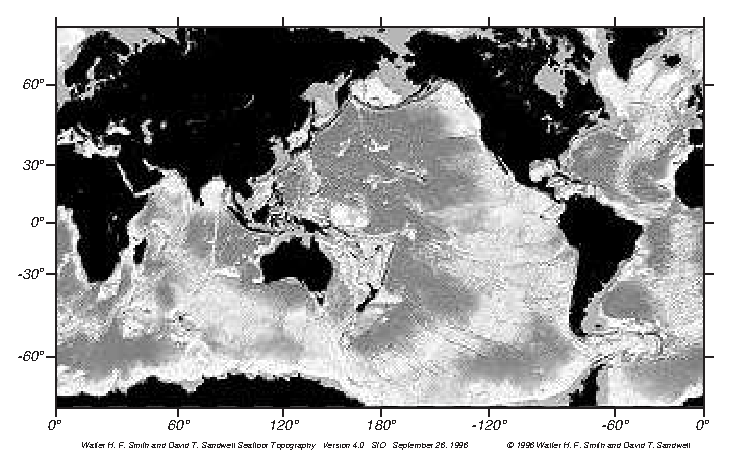
\includegraphics{pics/worldbathym}}
\caption{Карта глубин океана с разрешением~$3\km$, созданная по данным 
спутниковых альтиметрических наблюдений поверхности моря (Smith and Sandwell).}
\label{fig:worlsbathym}
\end{figure}

%% ??? в последней редакции PDF ссылок на этот рисунок нет.
%% кроме того, в новой редакции отсутствует разъяснение, что
%% > ... Несмотря на то, что значения на этой карте нанесены на пятимильную 
%% > сетку, данные использованные при её изготовлении часто имеют гораздо 
%% > большее пространственное разрешение, особенно в Южном Океане, 
%% > где расстояния между маршрутами кораблей в некоторых регионах может 
%% > достигать 500 км.
%% Без него становится непонятной оговорка в разделе 2.5 об осторожности с
%% выбором массивов данных.

Правительства разных стран публикуют карты побережья и гаваней. В США за эту
деятельность отвечает NOAA National Ocean Service, которая выпускает 
навигационные карты гаваней и вод материковой отмели.
%% offshore waters = "вод материковой отмели"
%% http://www.multitran.ru/c/m.exe?CL=1&l1=1&s=offshore+waters
%% но еще и "открытого моря" (там же).
%% кроме того, материковая отмель --- уж не континентальный ли это шельф?
%
% National governments publish coastal and harbor maps. In the USA, the
% \textsc{noaa} National Ocean Service publishes nautical charts useful for
% navigation of ships in harbors and offshore waters.
\end{section}

\begin{section}{Звук в океане}
% \section{Sound in the Ocean}
Звук обеспечивает единственный приемлемый способ передачи информации
на большие расстояния в океане. При помощи звука измеряются характеристики
дна океана и его глубина, а также температура и параметры течений. Киты и
другие животные, обитающие в океане, используют звук для навигации, общения
друг с другом на больших расстояниях и поиска пищи.
%% уместно ли говорить "навигация" по отношению к китам? Они штурманских 
%% классов не заканчивали.
%
% Sound\index{sound!in ocean} provides the only convenient means for 
% transmitting information over great distances in the ocean.
% Sound\index{sound!use of} is used to measure the properties of the sea 
% floor, the depth of the ocean, temperature, and currents. Whales and other
% ocean animals use sound to navigate, communicate over great distances,
% and find food.

%\paragraph{Sound Speed}
Скорость звука в воде зависит от температуры, солёности и 
давления (MacKenzie, 1981; Munk et al. 1995: 33):
\begin{equation}
\begin{split}\label{MacKenzieFormula}
  C & = 1448.96 + 4.591\,t - 0.05304\,t^2 + 0.0002374\,t^3+ 0.01630\,Z \\
    & + (1.340 - 0.01025\,t) (S - 35) + 1.675 \times 10^{-7}\,Z^2 
      - 7.139 \times 10^{-13}\,t\,Z^3
\end{split}
\end{equation}
где $C$~--- скорость в м/с, $t$~--- температура в градусах Цельсия, 
$S$~--- солёность (см.\ определение в гл.~6) в промилле
%% соленость в промилле (http://en.wikipedia.org/wiki/Sound_speed#Seawater)
и~$Z$~--- глубина в метрах. Точность этой формулы примерно~$0.1\mps$
(Dushaw, et al. 1993). Существуют и другие популярные формулы скорости звука,
например, формула Вильсона Wilson (1960), которую широко использовал
военно-морской флот США.
%
% The sound speed \index{sound!speed}in the ocean varies with
% temperature, salinity, and pressure (MacKenzie, 1981; Munk
% et al. 1995: 33):
% \begin{align}
%   C & = 1448.96 + 4.591\,t - 0.05304\,t^2 + 0.0002374\,t^3+ 0.0160\,Z \\
%   &+ (1.340 - 0.01025\,t) (S - 35) + 1.675 \times 10^{-7}\,Z^2 - 7.139 \times
% 10^{-13}\,t\,Z^3 \notag
% \end{align}
% where $C$ is speed in m/s, $t$ is temperature in Celsius, $S$ is salinity 
% (see Chapter 6 for a definition of salinity), and $Z$ is depth in meters.
% The equation has an accuracy\index{accuracy!equation!sound speed} of
% about 0.1 m/s (Dushaw et al. 1993). Other sound-speed equations have been
% widely used, especially an equation proposed by Wilson (1960) which has been
% widely used by the U.S. Navy.

В обычных условиях скорость звука~$C$ составляет от~$1450$ до~$1550\mps$ 
(рис.~\ref{fig:soundprofile}). 
Используя формулу~\ref{MacKenzieFormula}, мы можем оценить влияние на скорость 
звука небольших изменений температуры, глубины и солёности, часто
происходящих в океане. Так, скорость звука
изменяется на~$40\mps$ при увеличении температуры на~$10^\circ$~Цельсия, 
на~$16\mps$ при увеличении глубины на~$1000\m$ и на~$1.5\mps$ при
увеличении солёности на~1~промилле. Таким образом, основные причины
изменения скорости звука~--- это температура и глубина (давление). 
Изменения солёности слишком малы, чтобы оказывать существенное влияние.
%
% For typical oceanic conditions, $C$ is usually between 1450 m/s and 1550 m/s 
% (figure 3.15). Using (3.1), we can calculate the sensitivity of $C$ to 
% changes of temperature, depth, and salinity typical of the ocean. 
% The approximate values are: 40 m/s per 10\degrees C rise of temperature, 
% 16 m/s per 1000 m increase in depth, and 1.5 m/s per 1 increase in salinity. 
% Thus the primary causes of variability of sound 
% speed\index{sound!speed!variation of} is temperature and depth (pressure).
% Variations of salinity are too small to have much influence.

\begin{figure}[t!]
\makebox[121 mm][c]{\includegraphics{pics/sound_profile}}
\caption{Процессы, приводящие к возникновению в океане подводного звукового
канала. 
\textbf{Слева:} температура~$T$ и солёность~$S$, измеренные НИС 
\textit{Hakuho Maru} в северной части Тихого Океана (рейс KH-87-1, 
станция JT (\latlonmin{33}{52.90}{N}, \latlonmin{141}{55.80}{E}), 
28 января 1987~г.).
\textbf{В центре:} изменение скорости звука в зависимости от изменений 
температуры, солёности и глубины. 
\textbf{Справа:} график зависимости скорости звука от глубины; подводный
звуковой канал образуется в точке минимума, приходящейся на глубину 
около~$1\km$. (JPOTS Editorial Panel, 1991).}
\label{fig:soundprofile}
\end{figure}
%
% \begin{figure}[t!]
% \makebox[121 mm] [c]{\includegraphics{sound_profile}}
% \footnotesize
% Figure 3.15 Processes \rule{0pt}{4ex}producing the sound 
% channel\index{sound!channel} in the ocean.
% \textbf{Left:} Temperature $T$ and salinity $S$ measured as a function 
% of depth during the R.V. \textit{Hakuho Maru} cruise KH-87-1, station JT, 
% on 28 January 1987 at Latitude 33\degrees 52.90$'$ N, 
% Long 141\degrees 55.80$'$ E in the North Pacific.
% \textbf{Center:} Variations in sound speed\index{sound!speed!variation of} 
% due to variations in temperature, salinity, and depth.
% \textbf{Right:} Sound speed\index{sound!speed!as function of depth} as
% a function of depth showing the velocity minimum near 1 km depth which
% defines the sound channel\index{sound!channel} in
% the ocean. (Data from \textsc{jpots} Editorial Panel, 1991).
% \label{fig:soundprofile}
% \vspace{-3ex}
% \end{figure}

Если изобразить на графике скорость звука как функцию глубины, то мы
увидим, что её минимум приходится примерно на~$1000\m$ 
(рис.~\ref{fig:raypaths}). Водный слой, расположенный на этой глубине, 
получил за свои особые свойства название 
\emph{подводного звукового канала}.  Он присутствует во всех океанах, 
а в высоких широтах обычно выходит на поверхность.
%% в индекс добавить два различных сокращения: DSC/SOFAR
%
% If we plot sound speed\index{sound!speed!as function of depth} as a function 
% of depth, we find that the speed usually has a minimum at a depth around
% 1000 m (figure 3.16). The depth of minimum speed is called the
% \textit{sound channel}\index{sound!channel|textbf}. It occurs in
% all ocean, and it usually reaches the surface at very high latitudes.

Важность подводного звукового канала в том, что звук в нем может 
распространяться очень далеко, иногда проходя половину пути вокруг Земли. 
Кратко, принцип действия подводного звукового канала состоит в следующем: 
звуковые лучи, которые начинают выходить из канала, отражаются обратно 
к его центру. Лучи, распространяющиеся вверх под небольшими углами к 
горизонтали, отражаются книзу, а лучи, распространяющиеся вниз, отклоняются 
кверху соответственно (рис.~\ref{fig:raypaths}). Глубина канала изменяется
от~$10$ до~$1200\m$ в зависимости от местоположения.
%
% The sound channel\index{sound!channel} is important because sound in the
% channel can travel very far, sometimes half way around the earth. Here is 
% how the channel works: Sound\index{sound!rays} rays that begin to travel
% out of the channel are refracted back toward the center of the channel.
% Rays propagating upward at small angles to the horizontal are bent downward,
% and rays propagating downward at small angles to the horizontal are bent
% upward (figure 3.16). Typical depths of the chan\-nel vary from 10 m to
% 1200 m depending on geographical area.

\begin{figure}[t!]
\makebox[121 mm] [c]{\includegraphics{pics/raypaths}}
\caption{Распространение в океане звука от источника, расположенного вблизи
оси подводного звукового канала (Munk et al. 1995).}
\label{fig:raypaths}
\end{figure}
%
% \begin{figure}[t!]
% \makebox[121 mm] [c]{\includegraphics{raypaths}}
% \footnotesize
% \centering
% Figure 3.16 Ray paths of sound\index{sound!rays} in the ocean for a
% \rule{0pt}{3ex}source near\\the axis of the sound channel. 
% After Munk et al. (1995).
% 
% \label{fig:raypaths}
% \vspace{-3ex}
% \end{figure}

\begin{paragraph}{Поглощение звука водной средой.}
Поглощение звука (абсорбция) на единицу расстояния зависит от интенсивности 
звука~$I$:
\begin{equation}
dI = -k I_0 \, dx,
\end{equation}
где $I_0$~--- интенсивность до поглощения, а $k$~--- коэффициент
поглощения, зависящий от частоты звука. Решение данного уравнения:
\begin{equation}
I = I_0 \exp(-kx)
\end{equation}
Типичные значения~$k$ (в децибелах на километр) составляют: $0.08\dBpkm$
при~$1000\Hz$ и~$50\dBpkm$ при~$100\,000\Hz$. Децибелы считаются таким
образом: $\mbox{дБ} = 10 \log(I / I_0)$, где $I_0$~--- первоначальная мощность
звука, $I$~--- мощность звука после поглощения.
%
% Absorption of sound \index{sound!absorption of}per unit distance
% depends on the intensity $I$ of the sound:
% \begin{equation}
% dI = -k I_0 \, dx
% \end{equation}
% where $I_0$ is the intensity before absorption and $k$ is an absorption
% coefficient which depends on frequency of the sound. The equation has the
% solution:
% \begin{equation}
% I = I_0 \exp(-kx)
% \end{equation}
% Typical values of $k$ (in decibels dB per kilometer) are: 0.08 dB/km
% at 1000 Hz, and 50 dB/km at 100,000 Hz. Decibels are calculated from:
% $dB = 10 \log(I/I_0)$, where $I_0$ is the original acoustic power,
% $I$ is the acoustic power after absorption.

Например, пройдя расстояние~$1\km$, сигнал с частотой~$1000\Hz$ ослабнет всего
на~$1.8\%$: $I = 0.982 I_0$. На том же расстоянии сигнал с 
частотой~$100\,000\Hz$ уменьшится до~$I = 10^{-5} I_0$. Частота сигнала,
обычно используемого при эхолотировании морского дна, составляет~$30\,000\Hz$, 
и его затухание при прохождении от поверхности до дна и обратно незначительно.
%
% For example, at a range of 1 km a 1000 Hz signal is attenuated by only 
% 1.8\%: $I = 0.982 I_0$. At a range of 1 km a 100,000 Hz signal is reduced
% to $I = 10^{-5} I_0$. The 30,000 Hz signal used by typical echo sounders to
% map the ocean's depths are little attenuated going from the surface to 
% the bottom and back.

Сигналы очень низкой, менее $500\Hz$, частоты были зафиксированы в подводном
звуковом канале на расстоянии мегаметров. В 1960~г.\ звук частотой~$15\Hz$ от
взрывов в подводном звуковом канале у австралийского города Перт был слышен
около Бермудских островов; он прошёл почти полмира. 
Дальнейшие эксперименты показали, что сигнал частотой~$57\Hz$, посланный 
в подводный звуковой канал около острова Херд (\latlon{75}{E}, \latlon{53}{S}), 
может быть зафиксирован на Бермудах в Атлантике и в Монтерее (Калифорния) на
побережье Тихого океана (Munk et al. 1994).
%
% Very low frequency sounds in the sound channel\index{sound!channel}, 
% those with frequencies below 500 Hz have been detected at distances
% of megameters. In 1960 15-Hz sounds from explosions set off in the sound
% channel\index{sound!channel} off Perth Australia were heard in the sound
% channel near Bermuda, nearly halfway around the world. Later experiment
% showed that 57-Hz signals transmitted in the sound channel near Heard
% Island (75\degrees E, 53\degrees S) could be heard at Bermuda in the Atlantic
% and at Monterey, California in the Pacific (Munk et al. 1994).
\end{paragraph}

\begin{paragraph}{Использование звука}
Поскольку низкочастотные звуки распространяются на большие расстояния, 
военно-морской флот США в 1950-х разместил на дне океана систему микрофонов
как в глубоких, так и в мелких водах, подключив их к наземным станциям. Эта
система акустической разведки SOSUS (Sound Surveillance System), первоначально
предназначенная для слежения за подводными лодками, нашла немало и других
применений. Так, она использовалась для поиска и слежения за китами на
расстоянии до~$1\,700\km$, а также для обнаружения подводных вулканических
извержений.
\end{paragraph}
%
% \paragraph{Use of Sound}
% Because low frequency sound \index{sound!use of}can be heard at
% great distances, the US Navy, in the 1950s, placed arrays of
% microphones on the sea floor in deep and shallow water and
% connected them to shore stations. The Sound Surveillance System
% \textsc{sosus}, although designed to track submarines, has found
% many other uses. It has been used to listen to and track whales up
% to 1,700 km away, and to find the location of sub-sea volcanic
% eruptions.
%\end{paragraph}
\end{section}

\begin{section}{Основные концепции}
% \section{Important Concepts}
\begin{enumerate}
\item
Если уменьшить ширину океана до 8 дюймов, то его глубина в том же масштабе
будет соответствовать толщине листа бумаги. Благодаря этому, поля скорости 
в океане близки к двумерным, а вертикальные скорости гораздо меньше
горизонтальных.
%
% \item If the ocean were scaled down to a width of 8 inches it  would have
% depths about the same as the thickness of a piece of paper. As a result, the
% velocity field in the ocean is nearly 2-dimensional. Vertical velocities 
% are much smaller than horizontal velocities.


\item
Количество океанов равно трём.%
\remark{О различных точках зрения на этот вопрос см. примечание 
на стр.~\pageref{remark:threeoceans}.}
%
% \vitem There are only three official ocean.

\item
Объём воды превышает вместительность океанических бассейнов, так что океаны
затапливают побережье континентов, образуя континентальный шельф.
%
% \vitem The volume of ocean water exceeds the capacity of the ocean basins,
% and the ocean overflows on to the continents creating continental shelves.

\item
Измерение глубины океанов и составление карт морского дна производится на 
основе информации, полученной при помощи установленных на судах эхолотов.
Принцип действия эхолота состоит в измерении времени, требуемого звуковому
импульсу для прохождения от поверхности до дна и в обратном направлении.
Карты глубин имеют в некоторых регионах малое пространственное разрешение,
поскольку эти регионы редко посещатся кораблями, так что маршруты измерений
расположены далеко друг от друга.
%
% \vitem The depths of the ocean are mapped by echo sounders which measure
% the time required for a sound\index{sound!used to measure depth} pulse to
% travel from the surface to the bottom and back. Depths measured by ship-based
% echo sounders have been used to produce maps of the sea floor. The maps have
% poor horizontal resolution in some regions because the regions were seldom
% visited by ships and ship tracks are far apart.

\item
Еще одним способом измерения глубин служат спутниковые альтиметрические 
системы, которые профилируют форму поверхности моря. Элементы подводного
рельефа вызывают изменение гравитации в месте своего расположения, что,
в свою очередь, влияет на форму морской поверхности в этом районе.
У современных карт, основанных на спутниковых альтиметрических измерениях 
и данных эхолотирования, ошибка по глубине составляет~$\pm 100\m$, 
а пространственное разрешение~---~$\pm 3\km$.
%
% \vitem The depths of the ocean are also measured by satellite altimeter
% systems which profile the shape of the sea surface. The local shape of the
% surface is influenced by changes in gravity due to sub-sea features. Recent
% maps based on satellite altimeter measurements of the shape of the sea
% surface combined with ship data have depth accuracy of $ \pm $100 m and
% horizontal resolutions of $ \pm $3 km.

\item
Скорость звука в океане составляет обычно~$1480\mps$ и определяется, в
основном, температурой, меньше~--- давлением, и совсем мало~--- 
солёностью. Зависимость скорости звука от температуры и глубины
создаёт в океане подводный звуковой канал, в котором звук может
путешествовать на огромные расстояния. Так, сигнал частотой менее~$500\Hz$
может обойти полмира при условии, что на его пути не встретится суша.
%
% \vitem Typical sound\index{sound!speed!typical} speed in the ocean is 
% 1480 m/s. Speed depends primarily on temperature, less on pressure, and very
% little on salinity. The variability of sound speed as a function of pressure
% and temperature produces a horizontal sound channel in the ocean. Sound in
% the channel can travel great distances. Low-frequency sounds below 500 Hz
% can travel halfway around the world provided the path is not interrupted
% by land.
\end{enumerate}
\end{section}

\end{chapter}
